\documentclass[12pt]{article}

% Minimal margins
\usepackage[a4paper, top=2cm, bottom=2cm, left=1.3cm, right=1.3cm]{geometry}

% Encoding and fonts
\usepackage[utf8]{inputenc}
\usepackage[T1]{fontenc}
\usepackage[english]{babel}
\usepackage{lmodern}
\usepackage{microtype}

% Spacing and layout
\usepackage{setspace}
\onehalfspacing

\usepackage{amsmath} % Erweiterung für den Mathe-Satz

% Figures and tables
\usepackage{graphicx}
\usepackage{caption}
\usepackage{subcaption}
\usepackage{booktabs}

\usepackage{dirtree}

\usepackage{url} % Dient zur Auszeichnung von URLs; setzt die Adresse in Schreibmaschinenschrift.
\usepackage{hyperref} % Links und Verweise werden innerhalb von PDF Dokumenten erzeugt

\usepackage{csquotes} % Kontextsensitive Zitiermöglichkeiten

\usepackage[backend=biber, style=ieee]{biblatex} % Bibliographie erstellen durch BibLaTex und Biber mit Zitationsstil IEEE
\addbibresource{Literature.bib} % Einlesen der aus Citavi ausgegebenen BibTex-Datei

% Custom section spacing (optional)
\usepackage{titlesec}
\titlespacing{\section}{0pt}{12pt}{6pt}
\titlespacing{\subsection}{0pt}{10pt}{4pt}

\usepackage{xcolor}
\newcommand{\red}[1]{{\color{red}#1}}

\title{Glomerulus segmentation from whole-slide images (WSIs)}
\author{Lukas Göbl, Peer Schäfer, Lukas Scheib}
\date{\today}

\begin{document}

\begin{titlepage}
    \centering
    \maketitle

    \vspace{2cm}

    % Images
    \includegraphics[width=0.9\textwidth]{Images/smol_good.png} \\
    \vspace{1cm}
    \includegraphics[width=0.9\textwidth]{Images/big_good.png}

    \vspace{0.5cm}

    % Caption for both images
    \captionsetup{type=figure, font=small}
    \begin{center}
        \caption*{Example predictions of our best models (Top: Experiment 4; Bottom: Experiment 5)}
    \end{center}
\end{titlepage}

\section{Introduction}

In our project we addressed the tasks of segmenting glomeruli from whole-slide and patch-level kidney biopsy images as part of the MICCAI 2024 Kidney Pathology Image segmentation (KPIs) Challenge on medical image segmentation. The core objective was to accurately identify glomerular structures, which is critical for diagnosing kidney diseases. Given the highly imbalanced nature of the data and the large image sizes, standard segmentation models tend to underperform.

In our work, we implemented and evaluated our \texttt{VariableUNet} architecture to primarily tackle the patch-level segmentation task. Our focus was on improving recall and $F_1$-score rather than accuracy, as the class imbalance rendered the latter misleading. We used a training and evaluation strategy using patch-based inference and a mix of a BCE and dice loss function (BCEDiceLoss). Despite finetuning our hyper parameters we only achieved a dice score of $74\%$, falling behind of the winning submissions. For the whole-slide segmentation task, we only implemented a strategy to patch the large images, but did not conduct any further experiments. Our implementation and results are available on \href{https://github.com/LScheib/cv25-glom-segmentation-from-wsis}{GitHub}.

% ---------------------- STATE OF THE ART ----------------------
\section{State of the art}

The KPIs 2024 Challenge introduced a large PAS-stained multi-species dataset with over 10,000 annotated glomeruli, highlighting the difficulty of scaling patch-level performance to whole-slide inference \cite{Deng.11.02.2025}. Top submissions used hybrid models consisting of CNNs and transformers, achieving Dice scores >94\% \cite{Deng.11.02.2025}.

Despite growing interest in transformers and hybrid models, U-Net variants remain a dominant choice due to their simplicity, modularity, and strong performance. Enhancements like attention gates \cite{Oktay.11.04.2018}, atrous spatial pyramid pooling \cite{Kim.26.07.2023}, and dilated convolutions \cite{Wang.07.04.2020} improve focus, multi-scale feature extraction, and receptive field size. These improvements have consistently boosted performance in patch-based glomerular segmentation. These techniques show that U-Nets remain highly competitive - particularly when adapted to domain-specific renal histology datasets.

\section{Patch-level segmentation task}
The primary objective of this task is semantic segmentation — that is, to predict a binary mask for each input patch, indicating the exact pixel boundaries of glomeruli within the image.

\subsection{Data} \label{data}
The dataset used originates from PAS-stained whole-slide images (WSIs) of mouse kidney tissue, collected from four well-established preclinical rodent models of chronic kidney disease (CKD). These models include Normal (Control), 5/6 Nephrectomy (5/6Nx), Diabetic Nephropathy (DN) and NEP25. It includes 8.866 image patches, split into a training, a validation and testing set. Each patch is sized 2048x2048 pixels and extracted from the WSIs. The dataset is highly imbalanced, with glomeruli representing a small fraction of the total pixels in each patch e.g. we calculated the background-to-foreground pixel ratio to be approximately 23:1 in the training set. This imbalance poses a significant challenge for segmentation models, as they may learn to predict the majority class (background), leading to poor performance on the minority class (glomeruli).


\subsection{Method}

In this section, we describe the design choices behind our segmentation model, including its architecture, loss formulation, and key training parameters.

\subsubsection{Model architecture}
Our model architecture is based on a modified U-Net \cite{Ronneberger.18.05.2015}, drawing from several published approaches to glomerulus segmentation in histopathological images. We initially considered more recent architectures such as Mask2Former \cite{Cheng.02.12.2021} or UPerNet \cite{Xiao.26.07.2018}, as used in the winning solution \cite{Cap.07.11.2024} of the KPIs challenge~\cite{Deng.11.02.2025}. However, due to limited project resources and the expected implementation effort, we chose to adopt a U-Net variant instead, following recommendations from our computer vision tutors. Despite not achieving the best Dice scores in \cite{Cap.07.11.2024}, the U-Net remains a widely used and well-understood baseline for biomedical image segmentation tasks.

Further architectural inspiration came from Li et al. \cite{Li.2021}, who proposed a U-Net extension for segmenting glomeruli in frozen kidney donor sections. Specifically, we adopted their use of dilated convolutions in the bottleneck to enable multi-scale feature extraction, as well as the standard skip connections between encoder and decoder stages. In contrast to \cite{Li.2021}, however, we decided not to use transfer learning from pre-trained \texttt{VGG16} weights \cite{Simonyan.04.09.2014}. Instead, all network weights were trained from scratch on the KPIs challenge dataset.

In our implementation, the number of feature channels in each U-Net stage is scaled proportionally to the input patch size, relative to a reference resolution of $2048 \times 2048$ pixels. This design enables experimentation with different patch sizes without the need to manually adjust the network structure for each resolution. For internal reference, we refer to this variant as \texttt{VariableUNet}. To the best of our knowledge, this dynamic scaling strategy has not been explicitly explored in prior work, although similar ideas may have been considered in related contexts.

The architecture follows the standard encoder-decoder structure, with each block in the encoder and decoder consisting of two consecutive \texttt{Conv-BatchNorm-ReLU} layers - a pattern we refer to as \texttt{DoubleConv}. The bottleneck employs three parallel $3 \times 3$ convolutions with increasing dilation rates (1, 2, and 4) to capture features at multiple scales. Decoder layers use transposed convolutions for upsampling and concatenate the corresponding encoder features via skip connections. The final layer is a $1 \times 1$ convolution producing a single-channel output of raw logits, suitable for use with a sigmoid activation during inference or with \texttt{BCEWithLogitsLoss} during training.

\subsubsection{Loss function and hyperparameters}

Following the approach described by Moreau et al.~\cite{Moreau.2024}, we combined binary cross-entropy (BCE) loss $\mathcal{L}_{\mathrm{BCE}}$ with Dice loss $\mathcal{L}_{\mathrm{DICE}}$ to improve segmentation performance on strongly imbalanced glomerulus masks. The combined loss function was defined as 
\[
\mathcal{L} = \alpha\,\mathcal{L}_{\mathrm{BCE}} + (1 - \alpha)\,\mathcal{L}_{\mathrm{DICE}},
\]
where $\alpha$ denotes the weighting factor of the BCE component. This parameter - referred to as \texttt{bce\_weight} in our codebase - was treated as a tunable hyperparameter, with values ranging from $0.0$ to $1.0$ explored during experimentation.

Other important hyperparameters included the learning rate for the Adam optimizer (tested at $10^{-3}$, $10^{-4}$, and $10^{-5}$), along with the input patch size and number of training epochs, both of which were adjusted depending on the experiment stage. Additionally, we experimented with different values for the smoothing factor $\epsilon$ used in the Dice loss, where the loss is defined as
\[
\mathcal{L}_{\mathrm{DICE}} = \frac{2\,\mathrm{TP} + \epsilon}{2\,\mathrm{TP} + \mathrm{FP} + \mathrm{FN} + \epsilon}.
\]
In addition, we made use of the optional \texttt{pos\_weight} parameter in the BCE loss function to penalize false negative predictions more heavily, thereby compensating for the imbalance between glomerulus and background pixels. This scalar was varied in a range from 1 to 25. All experiments were conducted with a fixed batch size of 16.

\subsection{Experiments, evaluation, and results}

\subsubsection{Setup and procedure}

All experiments were conducted in PyTorch on an Nvidia A30 GPU with 24\,GB VRAM. We trained our model on the official KPIs challenge dataset using the predefined training, validation, and test splits, unless stated otherwise. In some experiments, however, we used only subsets of the training and validation data to obtain faster results during preliminary evaluations.

Initial experiments were conducted with smaller patches ($256 \times 256$ pixels) for faster iteration. Most final configurations were trained on full-size patches ($2048 \times 2048$) for 5{-}20~epochs, depending on their performance. While these numbers may seem low, training a single model for one epoch on the full-resolution dataset took approximately one hour due to the input size, model complexity, and dataset volume - resulting in runtimes of up to 20~hours per experiment.

Model optimization relied on the Adam optimizer with a fixed learning rate (typically Adam’s default value of $10^{-3}$), without a learning rate scheduler. The loss function was implemented as a weighted combination of BCE and Dice loss. We experimented with different values for the weighting factor \texttt{bce\_weight}, as well as the optional positive class weighting parameter \texttt{pos\_weight} in the BCE loss to compensate for class imbalance.

Performance was evaluated using accuracy, precision, recall, and $F_1$-score on the training, validation, and test sets. Note that for binary segmentation tasks, the Dice score and $F_1$-score are mathematically equivalent; we therefore use the term $F_1$-score consistently throughout this paper, even when referring to the primary challenge metric. In addition to the quantitative evaluation, selected configurations were qualitatively assessed via visual inspection of predicted segmentation masks.

\subsubsection{Experimental results}

Our initial training attempts began with a \texttt{VGG16}-based encoder pretrained on ImageNet, which was later discarded in favor of training from scratch to increase flexibility. Early experiments were hindered by a legacy normalization step and a data loading bug causing image-mask mismatches, which, once resolved, allowed the model to start identifying glomeruli.

Despite this, the model initially tended to predict only background, yielding superficially high accuracy (around $96\%$) due to the pronounced class imbalance discussed in section~\ref{data}. This observation motivated the use of the \texttt{pos\_weight} parameter to penalize false negatives more strongly.

We also explored architectural scaling by adjusting input patch sizes and proportionally scaling the number of channels in the U-Net. Setting the reference patch size to 2048 pixels proved critical to avoid GPU memory errors.

This initial phase established a functional model and data pipeline, paving the way for more systematic hyperparameter tuning and training experiments described below.

\paragraph{Experiment 1: Initial hyperparameter tuning}  
We started by exploring key hyperparameters including the weighting factor for the BCE loss (\texttt{bce\_weight}), the smoothing parameter for the Dice loss (\texttt{dice\_smooth}), and the positive class weighting parameter (\texttt{pos\_weight}) to address class imbalance. To reduce computational costs, all training runs in this experiment used reduced subsets consisting of 700 (shuffled) training and 50 validation samples.  

Training was conducted on full-size input patches ($2048 \times 2048$ pixels) with a fixed batch size of 16 for 5 epochs per configuration. The learning rate was kept constant at $10^{-3}$. Table~\ref{tab:exp1_top5} summarizes the top-performing hyperparameter combinations based on $F_1$-score, with a particular focus on recall, as most models tended to gravitate toward the majority class baseline.

\begin{table}[t]
    \centering
    \begin{tabular}{c|ccc|cccc}
        \toprule
        Rank & BCE weight & Dice smooth & Pos weight & Accuracy & Precision & Recall & $F_1$-score \\
        \midrule
        1 & 0.6 & 1e-06 & 1 & 0.9345 & 0.3383 & 0.5211 & 0.4103 \\
        2 & 0.8 & 1e-05 & 10 & 0.9176 & 0.2654 & 0.5004 & 0.3469 \\
        3 & 0.4 & 1e-04 & 25 & 0.8463 & 0.1558 & 0.5695 & 0.2447 \\
        4 & 0.8 & 1e-04 & 10 & 0.8123 & 0.1184 & 0.5108 & 0.1922 \\
        5 & 0.6 & 1e-06 & 25 & 0.6865 & 0.1058 & 0.8277 & 0.1875 \\
        \bottomrule
    \end{tabular}
    \caption{Exp. 1: Top 5 hyperparameter configurations with recall > 0.5, ranked by $F_1$-score. Metrics computed on validation data.}
    \label{tab:exp1_top5}
\end{table}


\paragraph{Experiment 2: Heatmap-based exploration}  
Building on the results of Experiment~1, we narrowed the hyperparameter ranges for \texttt{bce\_weight} and \texttt{pos\_weight} to values between 0.55{-}0.65 and 13{-}25, respectively. The Dice smoothing parameter was fixed at its best-performing value ($\texttt{dice\_smooth} = 10^{-6}$), as it showed little sensitivity in previous trials. Apart from that, we retained the same experimental setup as before in terms of training epochs, learning rate, batch size, and dataset size - except that a newly shuffled subset of the full training data was used.

The results were visualized as heatmaps depicting validation $F_1$-score and recall with respect to \texttt{bce\_weight} and \texttt{pos\_weight} (see Figure~\ref{fig:exp2_heatmaps}). Based on these heatmaps, and prioritizing recall while also considering $F_1$-score, we selected two promising configurations for further investigation in Experiment~3.

\begin{figure}[t]
    \centering
    \includegraphics[width=0.48\textwidth]{Images/12_heatmap_f1_score_by_weights.png}
    \includegraphics[width=0.48\textwidth]{Images/12_heatmap_recall_by_weights.png}
    \caption{Exp. 2: Heatmaps showing the effect of BCE weight and positive class weight on validation $F_1$-score (left) and recall (right).}
    \label{fig:exp2_heatmaps}
\end{figure}

\paragraph{Experiment 3: Full-patch training – first attempt} 
We selected two configurations from Experiment~2 that offered a favorable trade-off between recall and $F_1$-score. These were then evaluated using the full training dataset and again high-resolution input patches ($2048 \times 2048$ pixels), as already employed in previous experiments. Each model was trained for 20~epochs with a fixed learning rate of $10^{-3}$, a batch size of 16, and a Dice smoothing parameter of $10^{-6}$. The two configurations differed only in their values for \texttt{bce\_weight} and \texttt{pos\_weight}: config. A used \texttt{bce\_weight} = 0.6 and \texttt{pos\_weight} = 25, while config. B used \texttt{bce\_weight} = 0.65 and \texttt{pos\_weight} = 13.

Initially, both configurations showed promising results. However, over the course of training, performance sharply declined - particularly with respect to recall. This phenomenon, which we dubbed the \emph{Great Depression}, is visualized in Figure~\ref{fig:exp3_metrics_plot}, showing a pattern where recall drops dramatically while accuracy remains deceptively high. This indicates that the model regressed toward predicting background-only masks, leveraging class imbalance to optimize accuracy at the cost of true segmentation performance.

\begin{figure}[t]
    \centering
    \includegraphics[width=0.65\textwidth]{Images/Exp3_acc_prec_rec.png}
    \caption{Exp. 3: Evolution of accuracy, precision, and recall over 10 training epochs for config. A and B.}
    \label{fig:exp3_metrics_plot}
\end{figure}

\begin{table}[t]
    \centering
    \begin{tabular}{c|cc|cccc}
        \toprule
        Config & BCE weight & Pos weight & Accuracy & Precision & Recall & $F_1$-score \\
        \midrule
        A & 0.6 & 25 & 0.9692 & 0.9423 & 0.3284 & 0.4871 \\
        \midrule
        B & 0.65 & 13 & 0.9657 & 0.9313 & 0.2486 & 0.3925 \\
        \bottomrule
    \end{tabular}
    \caption{Exp. 3: Validation metrics after 10 epochs of the so far best-performing configurations.}
    \label{tab:exp3_metrics}
\end{table}

The unexpectedly poor results (as shown in table~\ref{tab:exp3_metrics}), together with the fact that all examined prediction masks were completely black - indicating that no glomeruli had been detected - prompted a thorough re-evaluation of the training pipeline. During this process, we discovered that a legacy normalization step, originally introduced for use with a now-discarded \texttt{VGG16} encoder, was still active in the \texttt{GlomDataset} class. Although this preprocessing did not appear to severely impair training, we removed it from all subsequent experiments to ensure consistency.

Up to this point, we had relied on Adam's default learning rate of $10^{-3}$. Given the observed instability during training on full-resolution data, we decided to revisit this choice and re-run future experiments with smaller learning rates, suspecting that the default setting may have been too aggressive for stable convergence.


\paragraph{Experiment 4: Focused re-tuning}  
Motivated by the failure cases observed in Experiment~3 and informed by recommendations from prior work~\cite{Moreau.2024}, we revisited the hyperparameter space with a more targeted and systematic approach. In particular, we reintroduced a \texttt{bce\_weight} of $0.8$ and explored configurations in the neighborhood of previously promising settings.

To accelerate this extended search, we reduced the input patch size to $256 \times 256$ pixels and trained all models on dataset subsets. Most configurations used 2000 training and 100 validation samples; for rapid prototyping, a few runs were performed on smaller subsets of 500 training and 50 validation samples.

Compared to earlier experiments, the following adjustments were made: smaller learning rates ($10^{-5}$ and $10^{-4}$) were explicitly tested in place of the Adam default ($10^{-3}$); \texttt{bce\_weight} was varied within a refined range of $\{0.6, 0.8\}$, while \texttt{pos\_weight} was tested at values $\{10, 15, 20, 25\}$; and \texttt{dice\_smooth} was primarily evaluated at $10^{-6}$ and $10^{-5}$, with one additional run at $10^{-3}$ to close a previously unexplored gap. Table~\ref{tab:top5_models_2} shows the top five configurations from this experiment with a recall of at least $0.5$, ranked by $F_1$-score and evaluated on the validation subset.

\begin{table}[t]
    \centering
    \begin{tabular}{c|ccc|cccc}
        \toprule
        Rank & BCE weight & Dice smooth & Pos weight & Accuracy & Precision & Recall & $F_1$-score \\
        \midrule
        1 & 0.8 & 1e-06 & 25 & 0.9774 & 0.7585 & 0.7713 & 0.7648 \\
        2 & 0.8 & 1e-05 & 20 & 0.9786 & 0.8048 & 0.7273 & 0.7641 \\
        3 & 0.8 & 1e-05 & 10 & 0.9781 & 0.8083 & 0.7080 & 0.7548 \\
        4 & 0.8 & 1e-05 & 25 & 0.9767 & 0.8036 & 0.6775 & 0.7352 \\
        5 & 0.6 & 1e-06 & 25 & 0.9749 & 0.8133 & 0.6166 & 0.7014 \\
        \bottomrule
    \end{tabular}
    \caption{Exp. 4: Top 5 hyperparameter configs with recall > 0.5, ranked by $F_1$-score on val. data.}
    \label{tab:top5_models_2}
\end{table}

\paragraph{Experiment 5: Final training run}  
In this final experiment, we selected the best-performing hyperparameter configuration from Experiment~4 and trained a single model on the entire dataset using full-size patches ($2048 \times 2048$). The aim was to verify whether the improvements observed during earlier small-scale evaluations would generalize under realistic training conditions.

The selected configuration used a high \texttt{bce\_weight} of 0.8 and a high \texttt{pos\_weight} of 25, combined with a very low \texttt{dice\_smooth} value ($10^{-6}$). The learning rate was explicitly set to $10^{-4}$.



Table~\ref{tab:exp5_metrics} summarizes the performance of this final model on both the validation and test sets. For comparison, we also report the performance of its smaller counterpart from Experiment~4, which was trained with identical model hyperparameters but on downscaled patches ($256 \times 256$ pixels instead of $2048 \times 2048$).

Interestingly, the smaller model achieved better performance overall. However, this comparison must be interpreted with caution: although test metrics for both models were computed on the full test set, the test images for the smaller model had to be downscaled prior to inference. As a result, the two setups are not strictly equivalent in terms of prediction difficulty. Qualitative results for both models are provided on the cover page and in the appendix.

\begin{table}[t]
    \centering
    \begin{tabular}{c|c|ccccc}
        \toprule
        Patch size & Split & Accuracy & Precision & Recall & $F_1$-score \\
        \midrule
        256 & Validation & 0.9781 & 0.7479 & 0.7660 & 0.7569 \\
          & Test       & 0.9757 & 0.7537 & 0.7133 & 0.7330 \\
        \midrule
        2048 & Validation & 0.9705 & 0.9299 & 0.3662 & 0.5255 \\
          & Test       & 0.9643 & 0.9159 & 0.2616 & 0.4070 \\
        \bottomrule
    \end{tabular}
    \caption{Exp. 5: Final evaluation metrics for two models with only differentiating patch sizes.}
    \label{tab:exp5_metrics}
\end{table}

\paragraph{Cross-Dataset evaluation on PanNuke}  
We positively confirmed the robustness of our model by evaluating its cross-domain generalization capabilities on the PanNuke dataset~\cite{Gamper.2019}, which provides multi-class nuclear annotations across a variety of tissue types. Since our model was trained for binary glomeruli segmentation, we converted the PanNuke ground truth masks into binary format by treating all non-background classes as foreground.

Given the lower spatial resolution of the PanNuke samples ($256 \times 256$ pixels), we adapted the training setup accordingly by reducing the patch size while keeping the hyperparameter configuration from Experiment~5 unchanged. The model was trained from scratch on Folds~1 and~2 of PanNuke, with Fold~3 reserved for validation. After 20 training epochs, the model achieved a validation $F_1$-score of 0.77, indicating decent performance despite the domain shift.

\subsubsection{Conclusion}

Through systematic iteration over architecture and training settings, we developed a U-Net-based segmentation model that achieves strong performance on the KPI glomerulus dataset, especially when trained on smaller input patches. Our experiments highlight that effective handling of class imbalance - via tuning of the \texttt{bce\_weight} and \texttt{pos\_weight} parameters - is crucial for achieving high recall in this domain.

While we successfully identified hyperparameter settings that performed well on $256 \times 256$ patches, these configurations did not generalize to larger input resolutions. This suggests that optimal settings on small patches do not directly translate to full-resolution training, likely due to differences in context, feature scale, and learning dynamics. However, cross-dataset evaluation on PanNuke has confirmed that our architecture is feasible in principle.

Overall, our results underline the importance of targeted hyperparameter exploration and caution against assuming scale invariance in model behavior - even with seemingly stable training setups.

\section{Whole Slide Image (WSI) segmentation}

The second part of the challenge focused on segmenting glomeruli in full whole slide images (WSIs) corresponding to the image patches employed in the patch-level segmentation task. This task introduces additional considerable computational and methodological challenges due to the extreme resolution and large file sizes of the WSIs. The largest image in the dataset measured up to 70,722~$\times$~81,137 pixels, making it infeasible to process in a single pass using a conventional pipeline for training convolutional neural networks like our \texttt{VariableUNet} architecture. This necessitated a new handling strategy to efficiently manage memory and computational resources.

\subsection{Implementation strategy}

Our approach was inspired by the winning submission of the challenge \cite{Cap.07.11.2024}, which utilized overlapping patches as a strategy for working with WSIs. Although alternative approaches exist for handling large WSIs—such as holistic histopathology \cite{Tang.03.07.2024} or visual prompting \cite{Wu.21.02.2024} strategies—patch-based inference remains a practical and widely adopted method. It aligns well with standard convolutional neural network pipelines and requires minimal architectural modifications.

\subsection{Hyperparameter choices}

The key hyperparameters in our WSI segmentation pipeline are the spatial dimensions of the patches (\texttt{patch\_size}    ) and the overlap of adjacent patches (\texttt{patch\_overlap}), where the size of the patches is independent of the patch overlap. The latter simply controls the stride of the patching operation. Additionally we introduce a trivial patch threshold (\texttt{threshold}) which is the minimum number of positive pixels required in a patch for it to be retained.

\subsection{Methodology}

In order to efficiently handle these large images without exceeding memory limits, we utilized the \texttt{OpenSlide} Python library. This library enables direct access to specific regions of a WSI file without loading the entire image into memory. By leveraging this functionality, we extract only the necessary patches for processing, significantly reducing RAM usage. Each extracted patch is saved with a filename that encodes the coordinates of its upper-left pixel within the original WSI. This metadata enables precise reconstruction of the full-resolution segmentation mask by stitching individual patches back together in their correct spatial locations.

To further optimize processing, we incorporated a preprocessing step that filters out trivial patches---those for which the segmentation mask is mostly background. We first load the patch mask and count positive pixels, i.e. pixels classified as glomeruli. We only save mask- and image patch pairs where the sum of positive pixels cross our threshold hyperparameter \texttt{threshold}. This reduces unnecessary computational load and prevents the model from learning from uninformative examples.

The WSI processing pipeline was implemented to work with a specific dataset structure containing the official \texttt{.tiff} files. This structure is listed in the appendix \ref{dirtree}. The resulting dataset is identical to the original patch-level dataset provided by the organizers of the challenge to seamlessly integrate into our segmentation pipeline.

\subsection{Results and observations}
The WSI processing pipeline was tested using a patch size of 2048 pixels, an overlap (i.e. stride) of 1024 pixels and a threshold of 1\,\% of the total pixel count.

The segmentation procedure generated a significantly larger number of patches compared to the original patch-level dataset. This increase in data volume stems from both the use of overlapping patches and possibly a smaller threshold for trivial patches. This results in patches that only contain a small number or only parts of glomeruli, as seen in the appendix \ref{threshold_image}.

Furthermore, the diversity of patches improved due to the shifting sliding window, which allowed glomeruli to appear in varying contexts and positions. This variation is expected to support better generalization during model training.

Overall, the segmentation logic performed as intended and proved capable of handling the complexities of full-slide processing. Due to the limited time frame of the project, it was not feasible to conduct an additional training experiment to empirically validate whether this more diverse dataset leads to improved model performance. However, this remains a promising direction for future research.

% ---------------------- DISCUSSION ----------------------
\section{Discussion}
% Summary (5 lines), what worked/didn’t (10 lines), perspectives/future work (5 lines)

Our work demonstrates that careful model design and loss function selection are essential for accurate glomerular segmentation in highly imbalanced medical images. Our \texttt{VariableUNet} with a dilated bottleneck and the BCEDiceLoss enabled substantial improvements in recall and $F_1$-score compared to naive baselines. We still surmise that our architecture might not be robust enough to generalize well since we could not find a hyperparameter combination that performs well on the full dataset.

The combination of BCE and Dice loss was crucial for overcoming the limitations of accuracy as a metric in imbalanced settings. Hyperparameter tuning, particularly for loss weights and positive class weighting, had a significant impact on model performance. Despite these improvements, our models exhibited considerable instability, with $F_1$-score and recall fluctuating significantly between epochs, even in later stages of training. This instability is likely attributable to the pronounced class imbalance and the sensitivity of the BCEDiceLoss to its hyperparameters. Furthermore, models that achieved promising results when trained on smaller subsets of the data often failed to generalize when trained on the full dataset, indicating potential overfitting or insufficient robustness to data variability.

In retrospect, placing greater emphasis on pre- and post-processing—such as downsampling and upsampling the patches—could have significantly improved our workflow. This approach might have accelerated training compared to our strategy of using full-size patches throughout. Future work could also focus on more advanced data augmentation or ensembling multiple models to further boost performance. Exploring transformer-based architectures or hybrid approaches like the top models of the challange may also help address the challenges of domain adaptation and generalization to unseen data.

%----------------------------------------------------------------------------
% Literaturverzeichnis
%----------------------------------------------------------------------------

% Literaturverzeichnis mit BibLaTeX
\printbibliography

% Alternativ: Literaturverzeichnis ohne BibLaTeX (dann auch oben ändern)
% \bibliography{Literatur}

\newpage

\appendix

\section{Example predictions of Experiment 4}

\includegraphics[width=0.9\textwidth]{Images/smol_bad.png}
\vspace{1cm}

\includegraphics[width=0.9\textwidth]{Images/smol_good.png}

\newpage

\section{Example predictions of Experiment 5}

\includegraphics[width=0.9\textwidth]{Images/big_bad.png}
\vspace{1cm}

\includegraphics[width=0.9\textwidth]{Images/big_semi_good.png}
\vspace{1cm}

\includegraphics[width=0.9\textwidth]{Images/big_good.png}

\newpage

\section{Example predictions on PanNuke dataset}

\includegraphics[width=0.9\textwidth]{Images/pannuke_bad.png}
\vspace{1cm}

\includegraphics[width=0.9\textwidth]{Images/pannuke_semi_good.png}
\vspace{1cm}

\includegraphics[width=0.9\textwidth]{Images/pannuke_good.png}

\newpage

\section{Expected file structure for WSI patching} \label{dirtree}

\dirtree{%
    .1 GlomDataset\_WSI/.
    .2 train/.
    .3 56Nx/.
    .4 12\_116/.
    .5 image\_wsi/.
    .6 12-116\_wsi.tiff.
    .5 mask\_wsi/.
    .6 12-116\_mask.tiff.
    .4 ..../.
    .3 .../.
    .2 .../.
}

\section{Example image of patches barely above threshold}

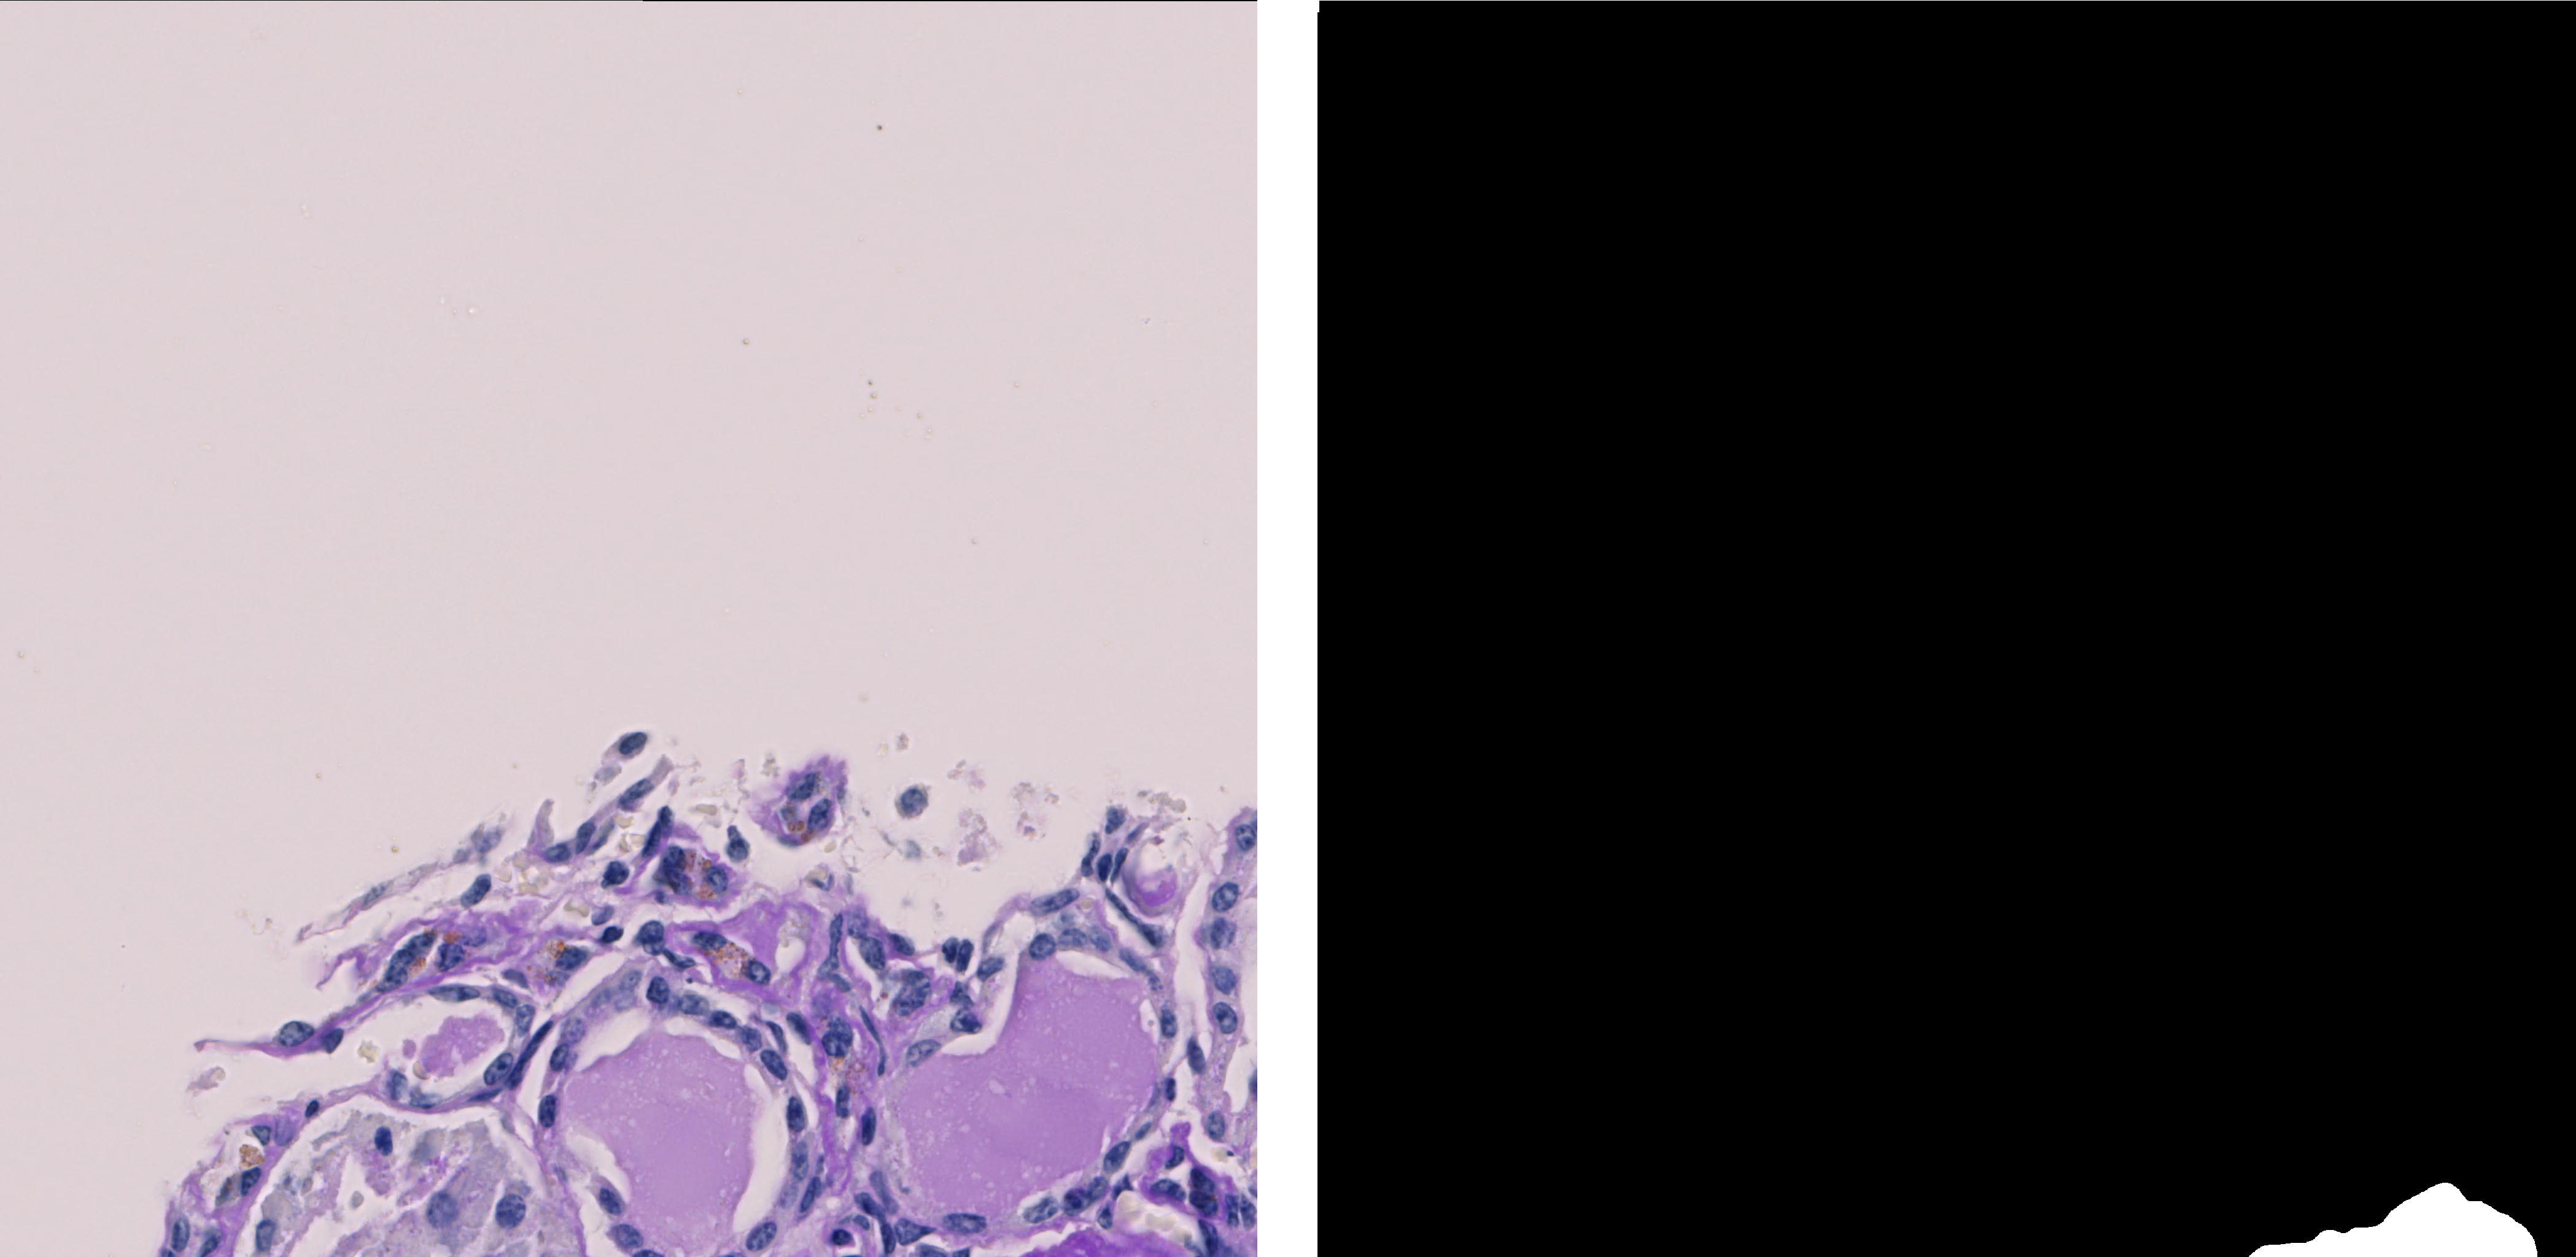
\includegraphics[width=0.9\textwidth]{Images/PatchBarelyAboveThreshold.png}\label{threshold_image}
\vspace{1cm}

\end{document}
